% --------------------------------------------------------------
% This is all preamble stuff that you don't have to worry about.
% Head down to where it says "Start here"
% --------------------------------------------------------------
 
\documentclass[12pt]{article}
 
\usepackage[margin=1in]{geometry} 
\usepackage{amsmath,amsthm,amssymb}
\usepackage[margin=1in]{geometry} 
\usepackage{amsmath,amsthm,amssymb}
\usepackage[T1]{fontenc} %escribe lo del teclado
\usepackage[utf8]{inputenc} %Reconoce algunos símbolos
\usepackage{lmodern} %optimiza algunas fuentes
\usepackage{graphicx}
\graphicspath{ {images/} }
\usepackage{tikz}
\usepackage[]{algorithm2e}
\usepackage{hyperref} % Uso de links
 
\newcommand{\N}{\mathbb{N}}
\newcommand{\Z}{\mathbb{Z}}
 
\newenvironment{theorem}[2][Theorem]{\begin{trivlist}
\item[\hskip \labelsep {\bfseries #1}\hskip \labelsep {\bfseries #2.}]}{\end{trivlist}}
\newenvironment{lemma}[2][Lemma]{\begin{trivlist}
\item[\hskip \labelsep {\bfseries #1}\hskip \labelsep {\bfseries #2.}]}{\end{trivlist}}
\newenvironment{exercise}[2][Exercise]{\begin{trivlist}
\item[\hskip \labelsep {\bfseries #1}\hskip \labelsep {\bfseries #2.}]}{\end{trivlist}}
\newenvironment{problem}[2][Problem]{\begin{trivlist}
\item[\hskip \labelsep {\bfseries #1}\hskip \labelsep {\bfseries #2.}]}{\end{trivlist}}
\newenvironment{question}[2][Question]{\begin{trivlist}
\item[\hskip \labelsep {\bfseries #1}\hskip \labelsep {\bfseries #2.}]}{\end{trivlist}}
\newenvironment{corollary}[2][Corollary]{\begin{trivlist}
\item[\hskip \labelsep {\bfseries #1}\hskip \labelsep {\bfseries #2.}]}{\end{trivlist}}

\newenvironment{solution}{\begin{proof}[Solution]}{\end{proof}}
 
\begin{document}
 
% --------------------------------------------------------------
%                         Start here
% --------------------------------------------------------------
 
\title{IADS Coursework 3: Heuristics for the Travelling Salesman Problem}


\maketitle
\newpage
\section*{C. Algorithm}
\subsection*{Motivation}
One of the simplest ways to construct an effective heuristic for TSP is to repeatedly apply small transformations to the current permutation and see how they affect the overall cost. Swap and 2-Opt heuristics are examples of this idea. My algorithm uses slightly more complicated transformations - it cuts the permutation in up to four places and considers combinations of putting the path back togetther. As only the ends of subpaths might get reconnected to different vertices, this transformation preserves most of the original solution.\\
\textbf{Notes:}\\
If improvement over a single iteration was less than 1$\%$, we switch to more cuts so that we perform more complex transformations only if simpler ones fail. Also, in each iteration we return a solution immediately if it is significantly better.

\subsection*{Pseudocode}

\begin{algorithm}[H]
 \KwData{perm}
 \SetKwData{Improvement}{improvement}\SetKwData{Perm}{perm}\SetKwData{Up}{up}
 \SetKwFunction{Union}{Union}
 \SetKwFunction{MyHeuristicIteration}{MyHeuristicIteration}
 \KwResult{best permutation found by the heuristic}
 $m_{opt} \leftarrow 1$ \;
 \For{$iterations \leftarrow 0$ \KwTo $30n$} {
  \Improvement, \Perm $\leftarrow$ \MyHeuristicIteration{$m_{opt}$}\;
  \uIf{improvement smaller than $0.1\%$ of current solution cost}{
   	increase $m_{opt}$ by 1\;
  }
  \uElse{
  	$m_{opt} \leftarrow 1$
  } 
 }
 \caption{Main method}
 
 
\end{algorithm}

\begin{algorithm}[H]
 \KwData{perm, $m_{opt}$}
 \SetKwData{Perm}{perm}
  \SetKwData{Improvement}{improvement}
  \SetKwData{Intervals}{intervals}
  \SetKwData{ReversedIntervals}{reversed-subpaths}
  \SetKwData{PermutedSubpaths}{permuted-subpaths}
  \SetKwData{NewTour}{new-tour}
  \SetKwData{BestTour}{best-tour}
   \SetKwFunction{Join}{Concatenate}
   \SetKwFunction{TourValue}{TourValue}
 \KwResult{best improvement found when cutting in $m_{opt}$ places (one iteration)}
 \BestTour $\leftarrow$ \Perm\;
 \ForAll{indices $i,j,k,l$ dividing perm  	\tcp*{some might be -1s, if $m_{opt} < 4$} } {
	\Intervals $\leftarrow$ \emph{subpaths after cutting the solution in $i,j,k,l$}\;
	\ForAll{\ReversedIntervals $\leftarrow$ possibilities of reversing some subpaths}{
		\ForAll{\PermutedSubpaths $\leftarrow$ possibilities of permuting \ReversedIntervals } {	
			\NewTour $\leftarrow$ \Join{\PermutedSubpaths}\;
			 \uIf{improvement bigger than $1\%$ of current solution cost}{
   				\KwRet{\NewTour}
   			 }
  			 
  			 \uElseIf {\TourValue{\NewTour} $<$ \TourValue{\Perm}} {
				\BestTour $\leftarrow$ \NewTour
			 }
		 }
	}
	\KwRet{\NewTour}
 }
 \caption{MyHeuristicIteration method}
\end{algorithm}
 
\subsection*{Time and memory complexity}
Let $n$ be the number of vertices in the graph.
\subsubsection*{Time complexity}
First, we are doing $\Theta(n)$ iterations.
Now, each iteration takes at most $O(n^5)$ time as for $m_{opt}=4$, we need to iterate over all possibilites to cut the permutation in 4 places (there are $n*(n-1)*(n-2)*(n-3)/4!$ of them) and for all such cuts we do $\Theta(n)$ work (there is a constant number of permutations, constant number of reversing subpaths).\\
Therefore, the total time complexity is $O(n^6)$.

\subsubsection*{Memory complexity}
The memory complexity is $O(n^2)$ as we need to maintain costs of edges and we do not need to maintain more than that at any time.

\section*{D. Experiments}

\newcounter{magicrownumbers}
\newcommand\rownumber{\stepcounter{magicrownumbers}\arabic{magicrownumbers}}

\begin{tabular}{|c|c|c|c|c|c|}
\hline 
 & Description & Swap & 2-Opt & Greedy & My heuristic \\ 
\hline
\rownumber & \begin{tabular}{@{}c@{}} 30 random points with coordinates\\ with magnitudes of 10 and less \end{tabular} & 257 & 101 & 115 & \textbf{99}\\
\hline
\rownumber & \begin{tabular}{@{}c@{}} 30 random points with $x \in <-10, 10>$\\ and $y \in <-10000, 10000>$ \end{tabular} & 120826 & \textbf{37385} & 37386 & \textbf{37385}\\
\hline
\rownumber & 
\begin{tabular}{@{}c@{}} 30 points placed evenly on a circle of radius 1000,\\ shuffled randomly \end{tabular} & 29025 & \textbf{6272} & \textbf{6272} & \textbf{6272} \\
\hline
\rownumber & \begin{tabular}{@{}c@{}} 5 per circle with radii: 1k, 2k, 4k, 8k + 5 random,\\sorted by distance from the origin \end{tabular} & 104617 & 68729 & 75383 & \textbf{64982} \\ 
\hline 
\rownumber & \begin{tabular}{@{}c@{}} 20 per circle with radii: 1k, 2k, 4k, 8k,\\sorted by distance from the origin \end{tabular} & 265427 & 117870 & 103379 & \textbf{101286} \\ 
\hline 
\rownumber & \begin{tabular}{@{}c@{}} 50 vertices with edge weights\\ chosen randomly from $<1,100>$ \end{tabular} & 1536 & 318 & 392 & \textbf{266}\\
\hline
\end{tabular}


\begin{enumerate}
\item As expected, heuristics that used more general transformations got better results (My heuristic had a smaller cost than 2-Opt and it, in turn, had a smaller cost than Swap).
\item Making the interval for y-s signifcantly wider increased the gap between Swap and the rest. As distances increase linearly with scaling, this wider gap should be caused by the increasingly worse relative quality of solutions that Swap yields. I have confirmed this with further tests (I have taken $y \in <-10^7,10^7>$).
\item Even though the points were shuffled, all but one heuristics managed to get the optimal solution (going along the circle). Therefore, this suggest that there are local minima which are significantly higher than the global minimum for swaps. The results for Swap and Two-Opt can be seen in Figure 1.
\item All other heuristics outperformed Swap again. From what I saw when I plotted the solution, it did not go stricly along the circles (and this state was a local minimum). My heuristic performed significantly better - I suspect this was due to the fact that it was able to do more complicated transformations and get itself out of more local minima.
\item This test is very similar to the previous one. What is interesting is that Greedy outperformed 2-Opt (as it followed the circles, because of its design). The results are visualised in Figure 2.

\end{enumerate}

\begin{figure}
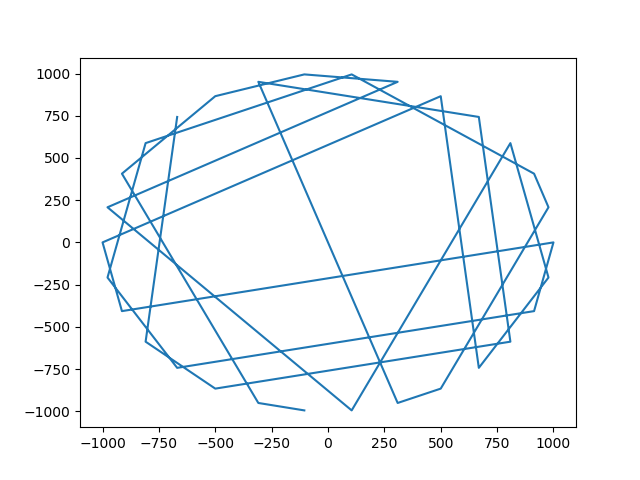
\includegraphics[scale=0.5]{CircleSwap.png}
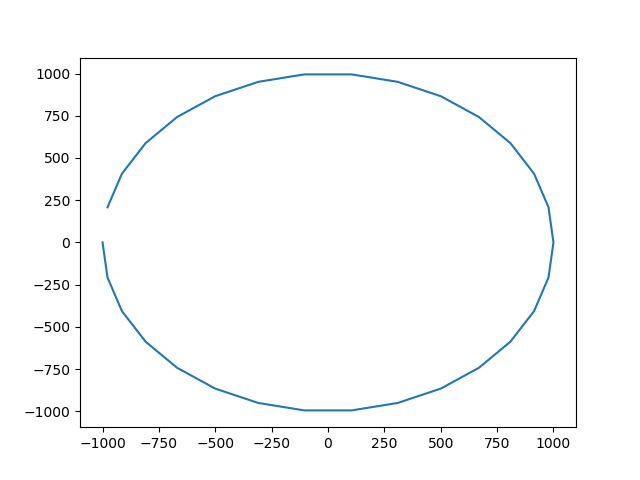
\includegraphics[scale=0.5]{CircleTwoOpt.png}
\caption{Swap and Two-Opt solutions for points placed evenly on a circle, shuffled}
\end{figure}

\begin{figure}
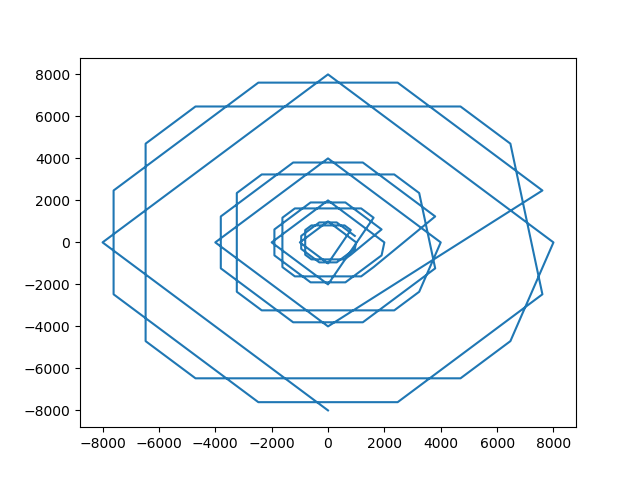
\includegraphics[scale=0.5]{20CirclesSwap.png}
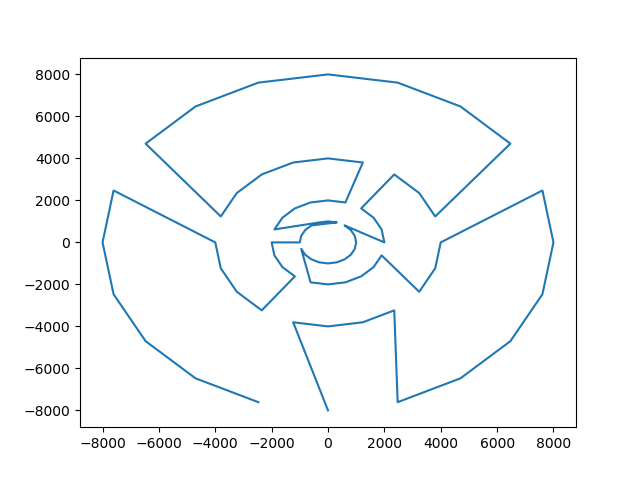
\includegraphics[scale=0.5]{20CirclesTwoOpt.png}
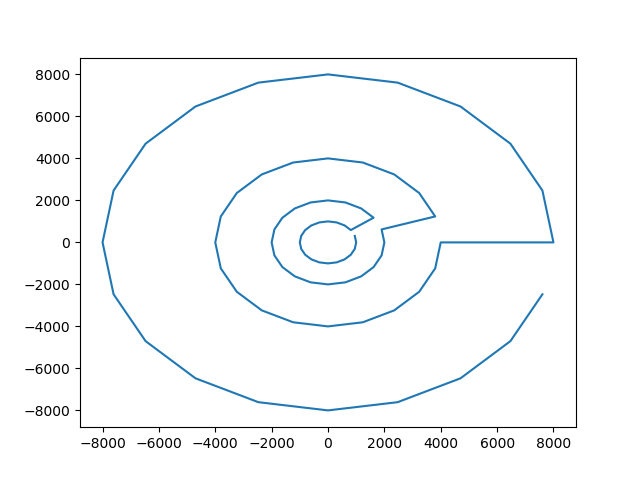
\includegraphics[scale=0.5]{20CirclesGreedy.png}
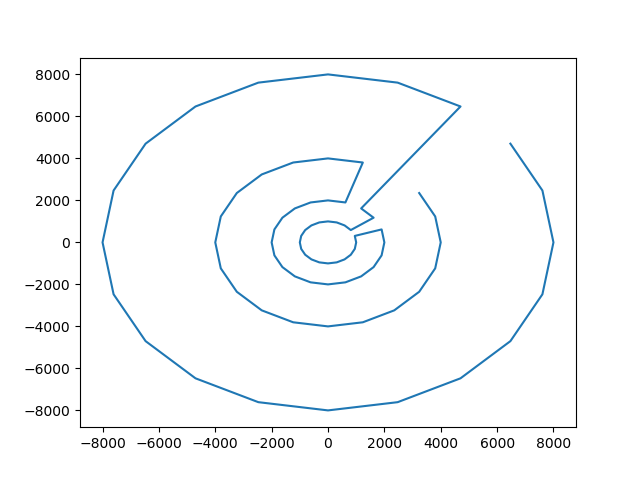
\includegraphics[scale=0.5]{20CirclesMyHeuristic.png}
\caption{Solutions for points placed evenly on 4 circles with radii 1000, 2000, 4000, 8000, initially sorted by distance from the origin (same order as in the table)}
\end{figure}

\end{document}

